% Farbkarte TU Darmstadt: http://www.webteam.tu-darmstadt.de/media/webteam_wissensdatenbank/artikel_1/farbkarte_TU_Darmstadt.png
\documentclass[nochapterpage,nopartpage,noheadingspace,numbersubsubsec,bigchapter,colorback,accentcolor=tud9c,10pt]{tudreport}
\usepackage[ngerman,english]{babel}

\usepackage[stable]{footmisc}
\usepackage[ngerman,english]{hyperref}

\usepackage{longtable}
\usepackage{multirow}
\usepackage{booktabs}

% Custom packages
\usepackage{wrapfig}
\usepackage{etoolbox}
\usepackage{multicol}
\usepackage{listings}

\lstset{
    breaklines=true,
    postbreak=\raisebox{0ex}[0ex][0ex]{\ensuremath{\color{red}\hookrightarrow\space}}
}

% Reset chapter counter after introducing a new part and start chapters on the same page
\makeatletter
\@addtoreset{chapter}{part}
\patchcmd{\scr@startchapter}{\if@openright\cleardoublepage\else\clearpage\fi}{}{}{}
\makeatother

\hypersetup{%
  pdftitle={Internet Praktikum TK Documentation},
  pdfauthor={M. Schanz},
  pdfsubject={Project Documentation},
  pdfview=FitH,
  pdfstartview=FitV
}

%%% Zum Tester der Marginalien %%%
  \newif\ifTUDmargin\TUDmarginfalse
  %%% Wird der Folgende Zeile einkommentiert,
  %%% werden Marginalien gesetzt.
  % \TUDmargintrue
  \ifTUDmargin\makeatletter
    \TUD@setmarginpar{2}
  \makeatother\fi
%%% ENDE: Zum Tester der Marginalien %%%

\newlength{\longtablewidth}
\setlength{\longtablewidth}{0.7\linewidth}
\addtolength{\longtablewidth}{-\marginparsep}
\addtolength{\longtablewidth}{-\marginparwidth}

\title{Internet Praktikum TK 2016\\ Conference Management System\\ Team Whisky}
\subtitle{Auel, Tarek,\\ Sahin, Huzeyfe\\ Schanz, Markus}


\begin{document}
\maketitle
\tableofcontents
%\listoffigures
%\addcontentsline{toc}{chapter}{\listfigurename}



\part{Technical Documentation}
\label{part:tech}

  \chapter{Introduction}
  \label{ch:tech:intro}

    This part of the documentation is intended for server administrators and/or developers who want to setup the project on their local machine. The documentation is written such that the individual chapters can be read in arbitrary order. Each chapter is a self-contained piece of documentation. However, the software tools listed in section~\ref{sec:tech:architecture:3rd-party} are heavily used throughout the application. Therefore, the reader is advised to read this section before proceeding with the rest of the documentation. For further information on these tools please refer to the individual project sites. Appendix~\hyperref[ch:appendix:setup]{A} hold the instructions on how to setup the application on a local machine.

    The remainder of this documentation is structured as follows: Chapter~\ref{ch:tech:architecture} gives an insight of how the application works conceptually and provides an overview of the used software libraries. Implementation details such as authentication, authorization, etc. are covered in chapter~\ref{ch:tech:implementation}. This also includes the directory structure of the project as well as important files that are involved in bootstrapping the application. Eventually, chapter~\ref{ch:tech:handson} describes the process of extending the application, i.e., how to extend the navigation, add a new page, etc.

  \chapter{Architecture}
  \label{ch:tech:architecture}

        \begin{figure}[!ht]
            \centering
            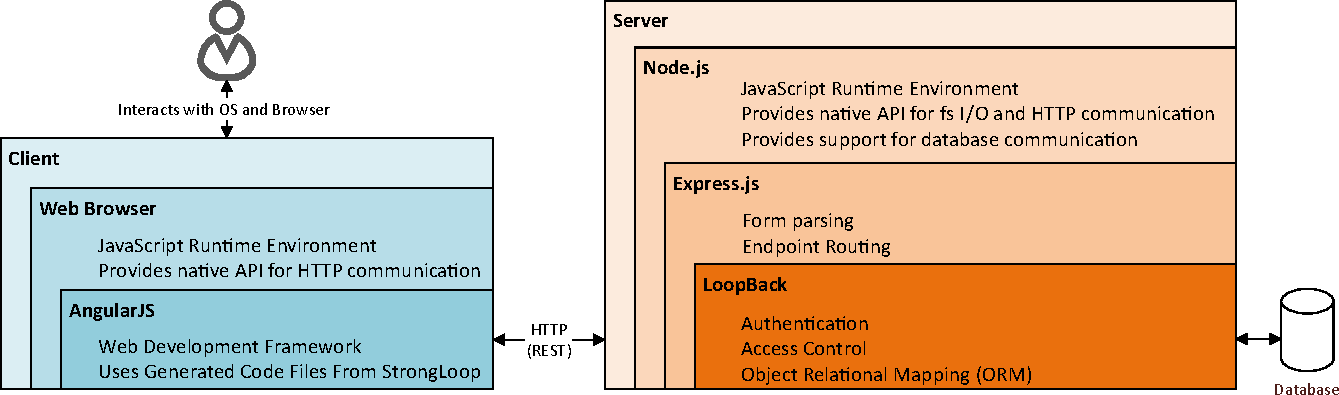
\includegraphics[width=\textwidth]{architecture-horizontal}
            \caption{Architecture.}
            \label{fig:architecture}
        \end{figure}

        %\begin{wrapfigure}{r}{0.5\textwidth}
        %\begin{figure}
        %    \centering
        %    \includegraphics[width=0.48\textwidth]{TUDreport-fig}
        %    \caption{In curley braces.}
        %    \label{fig:client-server}
        %\end{figure}
        %\end{wrapfigure}
  \section{Overview}
  \label{sec:tech:architecture:overview}
    On a high-level view, the application follows a client-server approach. The server part of the application primarily manages the database and provides a public REST API%
    \footnote{\url{https://en.wikipedia.org/wiki/Representational_state_transfer}}
    whereas the client part runs in the browser of the user and provides an user interface (UI). The client part is responsible to translates user interactions into requests against the server API and reflect the responses in the UI.

  \section{Third Party Software}
  \label{sec:tech:architecture:3rd-party}

    As seen in figure~\ref{fig:architecture}, the application utilizes third party software \& libraries in order to keep the codebase clean and allow for a productive development. This section gives an overview of the most important third party libraries \& tools that the project relies on.

  \paragraph{Node.js \& Node Package Manager}
    \emph{Node.js} is a standalone JavaScript runtime environment, i.e., it requires no web browser to execute JavaScript code.%
    \footnote{\url{https://nodejs.org/}}
    In recent years, \emph{Node.js} became very popular as it allows developers to use JavaScript for both server and client programming. It comes bundled together with its own package manager \emph{npm} which can be used to install a wide variety of third party libraries that further ease the development process.

  \paragraph{StrongLoop}
    \emph{StrongLoop} is a mandatory library on which the application is primarily build upon.%
    \footnote{\url{https://strongloop.com/}}
    This tool is able to generate code files for both server and client that can be used to manipulate a previously defined database schema. It comes bundles with a framework called \emph{LoopBack} and a library called \emph{Express.js} that is used internally to parse and route HTTP requests. It can be installed (and kept up-to-date) via \emph{npm}.

  \paragraph{Bower}
    Analogous to \emph{npm}, \emph{Bower} is a package manager for JavaScript libraries.%
    \footnote{\url{https://bower.io/}}
    However, \emph{npm} manages libraries that are required for the server part of the application (Node.js) whereas \emph{Bower} focuses on the management of libraries that are used on the client side, i.e., in the browser.

  \paragraph{AngularJS}
    AngularJS is a web application framework that eases web development by providing a model-view-controller (MVC) like architecture.%
    \footnote{\url{https://angularjs.org/}}
    The code that is generated by \emph{StrongLoop} is also targeting AngularJS.

  \chapter{Implementation}
  \label{ch:tech:implementation}

    % TODO: Introduction. This chapter covers the implementation details of the project.

  \section{Project Directory Structure}
  \label{sec:tech:implementation:dirs}

    The top level directory of the project is organized as follows:
        \begin{multicols}{4}
            \begin{itemize}
                \item /bin
                \item /client
                \item /common
                \item /doc
                \item /node\_modules
                \item /server
                \item /storage
            \end{itemize}
        \end{multicols}

  \paragraph{/}
    Besides the listed directories above, the root directory \emph{/} does also contain several files worth mentioning. \emph{bower.json} and \emph{.bowerrc} are the configuration files that are automatically found and loaded by \emph{Bower}. They contain the list of dependencies and corresponding version constraints to be installed by \emph{Bower}. By renaming the \emph{db.json.default} file to \emph{db.json}, the application can be tested with some predefined seed data. The \emph{package.json} file is to \emph{npm} what \emph{bower.json} is to \emph{Bower}. The other files in the directory are either self-explaining or irrelevant for this part of the documentation.

  \paragraph{/bin}
    Contains executable scripts that are used to initialize the application database with dummy data.

  \paragraph{/client}
    Resembles the root directory that is publicly accessible through the HTTP web server, i.e., it contains all the code that is relevant for the client application.

  \paragraph{/common}
    Holds the models that describe the application database schema. These models are taken into account by \emph{StrongLoop} when generating the client- and server code files. The files inside this directory can either be edited manually (according to a specified standard) or through the \emph{StrongLoop} console line interface.

  \paragraph{/doc}
    Contains all documentation relevant files such as the documentation at hand.

  \paragraph{/node\_modules}
    This is where \emph{npm} stores downloaded modules. Besides a \emph{.gitignore} file, this directory is empty when the repository is checked out cleanly.

  \paragraph{/server}
    Contains the code that is executed inside the Node.js environment on the server side. It provides the logic to manipulate data, handles authentication and access control and also provides the public REST API.

  \paragraph{/storage}
    \emph{LoopBack}\footnote{The framework provided by \emph{StrongLoop}} manages file uploads in so-called containers. This directory contains one directory for each container and each of these hold in turn a list of files that were uploaded to the corresponding container. This directory is initially empty when the repository is checked out cleanly. It gets filled once the conference users start to submit their papers.

  \section{Entry Scripts}
  \label{sec:tech:implementation:bootstrapping}

    Entry scripts are the first step in the bootstrapping process of the application. These are somewhat comparable to the \emph{main()} method of a \emph{C++} program. Since the application runs in a distributed fashon, i.e., on a client and a server, it has entry scripts for both of them.

  \subsection{Server Application}
  \label{sec:tech:implementation:bootstrapping:server}

    As described in section~\ref{sec:tech:implementation:dirs}, the server part of the application resides inside \emph{/server}. When \emph{Node.js} is started inside the project root directory via \texttt{node .}, it executes the script \emph{server/server.js}, as defined in \emph{package.json}. Like most of the files inside \emph{server/}, this file is in large parts the unmodified version of the \emph{LoopBack} example application.%
    \footnote{\url{https://github.com/strongloop/loopback-example-passport}}. It setups some preliminary routes for \emph{Express.js} as well as configuring some middleware components, e.g. to parse form data. Eventually, the start-up routine runs and forwards all requests to \emph{LoopBack} which than handles the request accordingly.

    The purpose of \emph{StrongLoop} is to provide a REST API to do basic CRUD\footnote{Create/Read/Update/Delete operations on a persistent storage} operations on a predefined database schema. Since all the magic is done by \emph{StrongLoop}, a developer usually does not need to dive further into the topic of request handling etc. Everything that a developer needs to do is defining and/or extending the models inside \emph{/common/models} and \emph{StrongLoop} will take care of the rest. The process of model creation and modification is described later in section~\ref{sec:tech:implementation:strongloop:models}.

  \subsection{Web Application}
  \label{sec:tech:implementation:bootstrapping:web}

    As previously mentioned~(\ref{sec:tech:implementation:dirs}), the \emph{/client} directory is exposed through the HTTP web server. In particular, the client is eventually sending an HTTP request to the root of this directory. Because no particular file is requested by the client, the server will respond with the contents of the \emph{index.html} file.

    The \emph{index.html} file consists of a simple HTML5 skeleton which basically includes lots of CSS and JavaScript files. Besides a lot of other scripts, the \emph{AngularJS} library is loaded. Once the browser is done with parsing the page and loading all embedded JavaScript files, the \emph{AngularJS} framework is scanning for an \texttt{ng-app} attribute inside the DOM. When found, AngularJS automatically starts its bootstrap routine and eventually executes the application, which happens to be defined inside \emph{js/app.js}. Section~\ref{sec:tech:implementation:angularjs} covers the contents of this file.

  \section{StrongLoop}
  \label{sec:tech:implementation:strongloop}

    As explained in section~\ref{sec:tech:architecture:3rd-party}, \emph{StrongLoop} is the tool that the application uses to abstract the manipulation operations on the database. Besides serving as an ORM, the application makes also use of its other features such as authentication, access control and file upload support. The application is mainly managed by the command line tool, \texttt{slc}, that comes together with \emph{StrongLoop}. It allows to generate and extend models, define access control rules and many more things. For an exhaustive description of the tool please refer to the documentation.\footnote{\url{https://docs.strongloop.com/display/public/LB/Command-line+reference}}

  \subsection{Creating and Updating Models}
  \label{sec:tech:implementation:strongloop:models}

    \emph{StrongLoop} does represent database tables in terms of models. A model does represent a collection of data with a given schema, e.g., a collection of users that have properties like a name, an email, a password, etc. Besides the sheer representation of data, the developer can define access rules in the model that define which data can be accessed by whom. In particular, this feature allows to restrict data access to the owner of the data. That said, a model does also provide the methods required to retrieve, store, update and delete items of a collections.

    To update or create a model, one has to decide between two basic approaches, i.e., a guided and a manual one. The advantages and disadvantages of both approaches are described next.

  \paragraph{Guided Approach}
    In the guided approach, the user can use the command line tool of \emph{StrongLoop} to extend or create models. In particular, the tool is capable of creating models (\texttt{slc loopback:model}), add properties to an existing one (\texttt{slc loopback:property}), associate ACL\footnote{ACL stands for access control list} rules (\texttt{slc loopback:acl}) and add relations\footnote{Possible relation types are HasOne, BelongsTo, HasMany, HasManyThrough and HasAndBelongsToMany} (\texttt{slc loopback:relation}). The main advantage of this approach is that it is easy to use and does not require the knowledge of the internal configuration format. In most parts it can be used intuitively without reading the documentation.

  \paragraph{Manual Approach}
    In the manual approach, the user has to edit the model directly inside the editor. This approach is useful for advanced ACL-, property- or relation-declarations. The command line tool does only generate basic code which is not sufficient for some use cases. In these cases, the user can use a hybrid approach in which he generates the basic code with the help of the command line tool and edit it manually afterwards. Please refer to the official \emph{StrongLoop} documentation for further information regarding the model format.\footnote{\url{https://docs.strongloop.com/display/public/LB/Defining+models}}

  \subsection{File Upload}
  \label{sec:tech:implementation:strongloop:container}

    The \emph{LoopBack} framework that comes with \emph{StrongLoop} does provide the ability to persist uploaded files from users. It does so by managing a set of so-called \emph{containers}. Basically, a container corresponds to a directory on a typical file system. When uploading a file, the user (or the application) has to define the container in which he wishes to upload it. The REST API generated by \emph{StrongLoop} does provide a special endpoint in order to download and upload files from a container.

    Containers must be defined inside the \emph{server/datasources.js} file. The application at hand does define a single container that is configured to store uploaded files on the local file system inside the \emph{storage/} directory. It does also rename the files according to a unique naming schema which ensures that files, once uploaded, cannot be overridden anymore. The defined container is used to store the PDF documents that are uploaded by the authors during the submission phase.

  \subsection{Generate AngularJS Services}
  \label{sec:tech:implementation:strongloop:genlib}

    It is important to remember that the application is distributed into a client and a server part. When adding or changing a model definition inside the \emph{common/models/} directory, the server part of the application just needs a restart in order to load the new model definitions. However, the part of the application that runs in the browser has no access to that directory. Instead, \emph{StrongLoop} is able to generate a set of AngularJS services, one for each model, that can be used inside the client. Whenever a model is added or changed, \emph{StrongLoop} has to re-generate that services. This is done by executing the following command inside the root of the project directory:
        \begin{lstlisting}[language=bash]
    $ lb-ng server/server.js client/js/services/lb-services.js
        \end{lstlisting}
    Please refer to the official documentation on more information about the command and automatic service generation.\footnote{\url{https://docs.strongloop.com/display/public/LB/AngularJS+JavaScript+SDK\#AngularJSJavaScriptSDK-GeneratingAngularservices}}

  \paragraph{Side Note}
    When starting to write code and using models, note that the usage of model classes on the server differs from that of the client. While the methods basically remain the same, the accepted arguments usually differ. For new developers this can be a confusing fact which is why this disclaimer has been placed here.

  \section{The AngularJS Client Application}
  \label{sec:tech:implementation:angularjs}

    As mentioned in section~\ref{sec:tech:architecture:3rd-party}, the generated code of \emph{StrongLoop} is targeting the \emph{AngularJS} web framework. The choice of using \emph{StrongLoop} therefore also implies the usage of AngularJS. The aim of this chapter is to provide a rough overview of how \emph{AngularJS} influences the development workflow of the application. After reading this section, the reader should be familiar with the application organization and be able to understand the basic concepts of \emph{AngularJS}.

  \subsection{The \texttt{app} Module}
  \label{sec:tech:implementation:angularjs:app}

    Inside the \emph{index.html} file, the body tag is defined as \texttt{<body ng-app="app">}. This instructs AngularJS to invoke the module called "app" and execute it. In order to let AngularJS know what to do, the "app" module must be defined and configured in advance. This is done inside the \emph{js/app.js} script. The task of this script is to
        \begin{itemize}
            \setlength\itemsep{0em}
            \item Setup the routes, i.e., the different "pages" that the user can visit. A route does not only consist of a location (URL address) but also of a view\footnote{A view is basically an HTML template that is embedded in the layout} and a controller that provides the logic behind the view.
            \item Define services that can be used by the controllers. Put simply, a service is a component with a single responsibility that can be accessed application-wide as a singleton instance. Services are most commonly used to abstract the communication between the application and the backend, e.g. to fetch or update data from an REST API. Services are identified by a unique name and can be accessed by controllers (see section~\ref{sec:tech:implementation:angularjs:controllers}) through that name.
            \item Define custom filters to transform raw data inside views into an appropriate representation. For example, a custom filter could be applied to the value 4\,239\,283 in order to interpret it as a file size, i.e., 4.04 MB. Filters help with sticking to the DRY programming principle and also to keep logic and complex statements separate from views.
            \item Configure third party services and modules. For example, the application uses the \emph{angular-permission}\footnote{\url{https://github.com/Narzerus/angular-permission}} library to handle access control inside the application according to the users competence (see section~\ref{sec:tech:implementation:acl:angular-permission}).
        \end{itemize}
    For further information on the concepts of AngularJS, please refer to their official documentation.\footnote{\url{https://docs.angularjs.org/guide/concepts}}

  \subsection{Controllers}
  \label{sec:tech:implementation:angularjs:controllers}

    % TODO: Add a figure to describe how controllers interact with the view and includes services
    In AngularJS a controller is usually associated with a view and is responsible to manage the logic behind it, i.e., it provides the data that is being displayed by the view and react to user interactions. The data exchange between the controller and the view happens implicitly through the built-in \texttt{\$scope} service\footnote{See section~\ref{sec:tech:implementation:angularjs:app} for a simple explaination of a service.} by using two-way data binding, i.e., whenever a value changes inside the view (through user interaction), the changes are reflected in the controller and vice versa. More information on controllers and the important concept of two-way data binding can be found in the official documentation.\footnote{\url{https://docs.angularjs.org/guide/controller} and \url{https://docs.angularjs.org/guide/databinding}}

    Controllers are defined inside the \emph{client/js/controllers/} directory.

  % TODO: Documentation is finished until here! (besides the TODO's)
  % The parts until the Hands On chapter require a revision
  \subsection{Layout and Templates}
  \label{sec:tech:implementation:angularjs:layout}

    Some more stuff.

  \section{Role Based Access Control (RBAC)}
  \label{sec:tech:implementation:rbac}

    There are user roles and access control

  \subsection{Roles}
  \label{sec:tech:implementation:acl:roles}

    Attendee, Author, Reviewer, Chair.

  \subsection{The \texttt{angular-permission} library}
  \label{sec:tech:implementation:acl:angular-permission}

    Describe how angular-permission is utilized to check for permissions.

  \chapter{Hands On: Extending the Application}
  \label{ch:tech:handson}

    This chapter describes the process of extending the web application by a new page that displays the current time to the user. This process involves ~\ref{sec:tech:handson:add-vc}) the creation of a view and its corresponding controller, ~\ref{sec:tech:handson:add-route}) the creation of a route and \ref{sec:tech:handson:navlink}) the modification of the navigation bar to include a reference to the newly created route. The instructions in this chapter will help to understand the basic patterns that are used throughout the whole application. Once understood, the application can be modified and extended with ease.

  \section{Creating a View and Controller}
  \label{sec:tech:handson:add-vc}

    The most natural way to start with the extension of the application is to create a new template that is going to display the current time to the user. All application templates are located inside \emph{client/views/}. Because the view is not going to require any special permission other than an authenticated user, it should be created inside \emph{client/views/user/}. While it is not required to follow any particular naming schema, it is common practice to name the view after the controller that is managing it. As our controller is going to be named \emph{TimeController}, the view file should be named \emph{time.html}. Speaking of which, the controller should reside inside the \emph{client/js/controllers/user/} directory respectively and be named \emph{time.js}.

  \paragraph{Template Content}
    Inside the newly created template, the following lines have to be added:
        \begin{lstlisting}[language=html]
    <div class="row">
        <div class="col-md-6 col-md-offset-3">
            <p>Hello, it is {{ time | date:'medium' }}</p>
        </div>
    </div>
        \end{lstlisting}
    The two \emph{div} containers are plain HTML markup syntax. The application uses the grid system of the bootstrap CSS framework\footnote{\url{http://getbootstrap.com/css/\#grid}}. The \emph{div} containers simple reduce the width of the area in which the content is displayed in half. The curly brace syntax (\texttt{\{\{ time | date:'medium' \}\}}) is recognized and interpreted by AngularJS. It basically outputs the value of the \emph{time} variable after passing it to a filter named \emph{date}. More on AngularJS template syntax and filters can be found in the official documentation.\footnote{\url{https://docs.angularjs.org/guide/templates} and \url{https://docs.angularjs.org/guide/filter}}

  \paragraph{Controller Content}
    The controller does only require a few lines of code as well. The following is enough to assign the desired value to the \emph{time} variable:
        \begin{lstlisting}
    angular.module('app').controller('TimeController', function ($scope) {
        $scope.time = new Date();
    });
        \end{lstlisting}
    These lines add a controller named \emph{TimeController} the the \emph{app} module that is managed by the angular framework. The second parameter of the \emph{controller()} method defines the function to be executed whenever this controller is invoked by angular. Also note the specified \emph{\$scope} parameter inside that function. This parameter will automatically be populated by AngularJS with the instance of the service with the same name. As mentioned earlier~(\ref{sec:tech:implementation:angularjs:controllers}) \emph{\$scope} is the name of a built-in service in AngularJS. It resembles the namespace that is implicitly made available to the view. More on controllers and the \emph{\$scope} service is found on the official documentation pages.\footnote{\url{https://docs.angularjs.org/guide/controller}}

  \section{Adding a new Route Definition}
  \label{sec:tech:handson:add-route}

    Now that the view and controller is created, AngularJS must be made aware of the fact that they belong together and also through which route (URL) they can be invoked.

  \paragraph{Include Controller inside index.html}
    In a first step, the newly created controller must be included by the browser when loading the application. Therefore, the following line has to be added to the \emph{index.html} file, alongside with the include statements of the other controllers:
        \begin{lstlisting}[language=html]
    <script src="js/controllers/user/time.js"></script>
        \end{lstlisting}

  \paragraph{Add Route Definition to app.js}
    The first \emph{.config()} call inside \emph{app.js} configures the \emph{\$stateProvider} which is part of the \texttt{ui-router} library.\footnote{\url{https://github.com/angular-ui/ui-router}}. A lot of \emph{state()} calls on the \emph{\$stateProvider} object configures the available routes of the application. On the bottom of this method chain, add the following lines:
        \begin{lstlisting}
    .state('app.protected.user.time', {
        url: '/time',
        templateUrl: 'views/user/time.html',
        controller: 'TimeController'
    })
        \end{lstlisting}
    This defines a new state which is inheriting any configuration options from its parent states, i.e. from the \emph{app}, \emph{app.protected} and \emph{app.protected.user} state. In particular, since it is defined as child of the app.protected state, it inherits the access permission (\texttt{permissions: \{ only: ['USER'] \}}) (see~\ref{sec:tech:implementation:acl:angular-permission}). Therefore, the newly created state will be available only to authenticated users. Also the defined url under which the state is going to be reachable will be expanded automatically to \texttt{/user/time}. For more information on states and configuration options, refer to the official documentation.\footnote{\url{https://github.com/angular-ui/ui-router/wiki}}

  \section{Add a Link to the Navigation Bar}
  \label{sec:tech:handson:navlink}

    Finally, the time has come to add a link to the navigation bar.
    extend layout where necessary (make a figure that describes the layout template and its embedded parts)

\part{User Documentation}
\label{part:user}

  \chapter{Introduction}
  \label{ch:user:intro}

    A conference management system...

  \chapter{Attendee}
  \chapter{Author}
  \chapter{Reviewer}
  \chapter{Chair}



\part{Appendix}
\label{part:appendix}

  \chapter*{A.\quad Application Installation}
  \addcontentsline{toc}{chapter}{A.\quad Application Installation}
  \label{ch:appendix:setup}

    The application does not enforce the usage of a specific operating system. However, we recommend to use a Linux system with a package manager in order to install the required prerequisites to make the setup process as smooth as possible.

  \section*{Prerequisites}
  \label{sec:appendix:setup:prerequisites}

    Before starting with the installation process, please make sure that your system does met the following prerequisites:
        \begin{multicols}{2}
        \begin{itemize}
            \item Git $\ge$ 2.x
            \item Node.js $\ge$ 4.2.x
            \item npm $\ge$ 3.x (part of Node.js)
        \end{itemize}
        \end{multicols}

    \noindent The project heavily relies on strongloop for generating API code as well as on bower to fetch 3rd party java-script libraries. To install both on your system execute the following command:
        \begin{lstlisting}[language=bash]
    # npm install -g strongloop bower
        \end{lstlisting}

  \section*{Installation}
  \label{sec:appendix:setup:install}

    \noindent Use the git command to fetch a copy of the source code repository.%
    \footnote{Requires read access to the repository.}
    The command should be executed by the user who is supposed to run the application and inside an empty directory which is going to hold the application source code.
        \begin{lstlisting}[language=bash]
    $ git clone ssh://git@scm.informatik.tu-darmstadt.de/iptk-ss2016/iptk-ss2016-team-whiskey.git .
        \end{lstlisting}
    For further installation instructions, please stick to the \emph{readme.md} file which is now found inside the directory.


  \chapter*{B.\quad Database Entity Relationship Model}
  \addcontentsline{toc}{chapter}{B.\quad Database Entity Relationship Model}

    % Figure of ERM goes here

  \chapter*{C.\quad Application Screenshots}
  \addcontentsline{toc}{chapter}{C.\quad Application Screenshots}

    % Figure of ERM goes here

  \chapter*{D.\quad (Un)Implemented Features}
  \addcontentsline{toc}{chapter}{D.\quad (Un)Implemented Features}

    % List of features goes here
    Below is the list of (un)implemented features, copied from the SCM wiki page.%
    \footnote{\url{https://scm.informatik.tu-darmstadt.de/projects/iptk-ss2016/wiki/Conference_management_system_-_Features}}
    A checked box ($\boxtimes$) means that the feature is implemented whereas an unchecked box ($\square$) means that the feature is (partly) unimplemented
        \begin{itemize}
            \setlength\itemsep{0em}
            \item Roles
            \begin{itemize}
                \item[$\boxtimes$] Authors [0..*]
                \item[$\boxtimes$] Reviewers [0..*]
                \item[$\boxtimes$] Chair [1..*]
            \end{itemize}

            \item General
            \begin{itemize}
                \item[$\boxtimes$] responsive design: access the web application with different kinds of devices (mobile, tablet, pc..)
            \end{itemize}

            \item As a user, I can
            \begin{itemize}
                \item[$\boxtimes$] register to the system at least with email, password
                \begin{itemize}
                    \item[$\boxtimes$] emails are unique
                    \item[$\boxtimes$] users can have multiple roles (e.g., author and reviewer)
                    \item[$\boxtimes$] additional information (see slides)
                    \begin{itemize}
                        \item[$\boxtimes$] e.g., basic profile (given name, family name, postal address)
                        \item[$\boxtimes$] e.g., affiliation (institution, city, state, country)
                    \end{itemize}
                \end{itemize}
                \item[$\boxtimes$] login to the system at least with registered email, password
                \item[$\boxtimes$] edit my profile (password, additional information)
                \item[$\boxtimes$] remove my profile
                \item[$\boxtimes$] logout
            \end{itemize}

            \item As a author, I can
            \begin{itemize}
                \item[$\boxtimes$] create a new submission (if submission is open)
                \begin{itemize}
                    \item[$\boxtimes$] title
                    \item[$\boxtimes$] registered authors [1..*] (given name, family name, email affiliation)
                    \item[$\boxtimes$] abstract
                    \item[$\boxtimes$] keywords (multi-selection) that describe the submission (e.g., research fields)
                    \item[$\boxtimes$] upload the paper (.pdf)
                \end{itemize}
                \item[$\boxtimes$] access current submissions (overview)
                \begin{itemize}
                    \item[$\square$] status: incompleted, completed, closed, accepted, rejected
                \end{itemize}
                \item[$\boxtimes$] look at a submission
                \item[$\boxtimes$] edit a submission (if submission is open)
                \item[$\boxtimes$] withdraw a submission
            \end{itemize}

            \item As a reviewer, I can
            \begin{itemize}
                \item[$\boxtimes$] access assigned submissions (overview + status)
                \item[$\boxtimes$] look at an assigned submission
                \begin{itemize}
                    \item[$\boxtimes$] details, pdf download or view
                \end{itemize}
                \item[$\boxtimes$] make a review > template (if review is open)
                \begin{itemize}
                    \item[$\boxtimes$] reviewer expertise: (1) not familar w/ the topic - (5) expert
                    \item[$\boxtimes$] overall evaluation: (1) strong reject - (5) strong accept
                    \item[$\boxtimes$] summary
                    \item[$\boxtimes$] major strong popints
                    \item[$\boxtimes$] major weak points
                    \item[$\boxtimes$] detailed comments
                \end{itemize}
                \item[$\boxtimes$] edit a review (if reviewing phase is open)
            \end{itemize}

            \item As a chair, I can
            \begin{itemize}
                \item[$\boxtimes$] list all paper submissions
                \begin{itemize}
                    \item[$\boxtimes$] look at a submissions (details, pdf download or view)
                    \item[$\square$] withdraw a submission
                \end{itemize}
                \item[$\boxtimes$] list all authors
                \begin{itemize}
                    \item[$\boxtimes$] look at detail information
                \end{itemize}
                \item[$\boxtimes$] list all reviewers
                \begin{itemize}
                    \item[$\boxtimes$] look at detail information
                \end{itemize}
                \item[$\boxtimes$] list all reviews
                \begin{itemize}
                    \item[$\boxtimes$] look at a review
                \end{itemize}
                \item[$\boxtimes$] assign papers to reviewers
                \begin{itemize}
                    \item[$\boxtimes$] conflict avoidance: an author is not allow to review his own paper
                \end{itemize}
                \item[$\boxtimes$] do the schedule management
                \begin{itemize}
                    \item[$\boxtimes$] automatic: set close deadlines for submissions and reviews
                    \item[$\boxtimes$] manual: (re-)open/close submissions and reviews
                \end{itemize}
                \item[$\square$] view fancy summary charts or reports (e.g., total submission, acceptances, topics, countries etc.)
            \end{itemize}

            \item Bonus features (OPTIONAL)
            \begin{itemize}
                \item[$\square$] users must confirm their registration by clicking on a registration link sent via email
                \item[$\square$] email notification to submitters and reviewers (status changes)
                \item[$\square$] chat with other online authors
                \item[$\square$] automatic assignment (even distribution) and conflict resolving
                \item[$\boxtimes$] a user can create multiple conference events and becomes the chair (=administrator) of them
            \end{itemize}
        \end{itemize}

\end{document}
